\documentclass[12pt,a4paper]{article}
\usepackage[utf8]{inputenc}
\usepackage[czech]{babel}
\usepackage[T1]{fontenc}
\usepackage[export]{adjustbox}
\usepackage{graphicx}
\usepackage{listings}
\usepackage{pdfpages}
\usepackage{float}
\usepackage{siunitx}
% proti vdove a syrotkovi
\clubpenalty 10000
\widowpenalty 10000

\begin{document}
%
%	TITLE
%
\begin{titlepage}
	
\includegraphics[left]{images/logo_fav}\par
	\vspace{5cm}
	{
		\centering
		\Huge{\textbf{Nápojový automat}}\\
		\Huge{\textbf{\textit{KIV/TI - Semestrání práce}}}\\
	}	
	\vfill
    \begin{tabular}{ll}
		vypracovali: & \it{Martin Matas, Martin Formánek, Tomáš Dubina} \\
		%studijní číslo: & A15B0089P \\
		%email: & martinm@students.zcu.cz \\
		datum: & {\large 27. listopadu 2016\par}
	\end{tabular}
\end{titlepage}
%
%	OBSAH
%
\tableofcontents
\newpage
%
%	TEXT
%
\section{Zadání}

\paragraph{\parindent=4em}{
	Vytvořte konečný automat pro řízení nápojového automatu. Automat bude mít tři typy vstupů: stisky tlačítek, indikaci hodnoty vhozené mince a signály z různých čidel (např. "došla káva", "došly kelímky" aj.). Svými výstupy bude automat řídit motory, elektromagnety apod., které zajistí vracení mincí z mincovníku, přípravu kelímku, ohřívání vody, napouštění vody apod. Konkrétní vnitřní prvky automatu si realisticky navrhněte sami.
}

\paragraph{\parindent=4em}{	
	Vytvořte dále aplikaci, která vhodným způsobem simuluje automat a umožňuje mačkání tlačítek, vhazování mincí a sledování vrácení přeplatku, rovněž by měla umožnit simulovat výjimečné stavy, např. "neteče voda" apod.
Hlavním smyslem zadání je vyzkoušet si návrh implementace pomocí konečného automatu.
}

\section{Teoretický rozbor}

\paragraph{\parindent=4em}{	
	Nápojový automat by měl zákazníkovi umožnit vhození mincí, nastavení množství cukru a volbu nápoje. Po objednání zvoleného nápoje musí automat vrátit případný přeplatek zákazníkovi. Automat by měl mít ošetřené vstupy před vhozením nepodporovaných mincí. Měl by nabízet pouze nápoje, ke kterým má všechny potřebné přísady, v případě, kdy automat nemá
	přísady pro přípravu nápoje, uvede se do stavu {\it Mimo provoz}. Pokud by došlo k výjimečnému stavu (např. odpojení přívodu s vodou), měl by automat umožnit zákazníkovi stornovat objednávku a vrátit peníze.
}

\newpage
\section{Teoretické řešení}

\subsection{Čidla automatu}

\begin{description}

\item [Externí] tlačítka pro výběr nápoje, tlačítka pro regulaci množství cukru, tlačítko pro stornování

\item [Interní] detekce vhození mince, přívod vody, detekce množství cukru, detekce počtu kelímků, detekce počtu směsí, detekce počtu mincí v mincovníku, čidlo hladiny vody v nádrži, čidlo teploty, pozice kelímku

\end{description}

\subsection{Vstupy programu}

\subsubsection{Externí}
\begin{description}

\item [Vstupní] ~
\begin{description}

\item [Impulsní] druh nápoje, přidání cukru, ubrání cukru, storno, vhození mince 1,2,5,10,20,50 Kč

\end{description}

\item [Výstupní] ~
\begin{description}

\item [Impulsní] výdej nápoje, vrácení přeplatku, zprávy na displeji - automat nemá na vrácení, indikace množství cukru, mimo provoz, nedostatek peněz pro nápoj, nedostatek směsi pro nápoj, zobrazení sumy vhozených mincí, nedostatek cukru, stornováno, odeberte nápoj, nápoj se připravuje, automat byl spuštěn

\end{description}

\end{description}

\subsubsection{Interní}
\begin{description}

\item [Vstupní] ~ 

\begin{description}

\item [Impulsní] přísun vody, poloha kelímku

\item [Hladinové] minimum cukru, výchozí množství cukru, maximální povolené množství cukru, maximální možné množství cukru, indikátory pro druh směsi, teplota vody, hladina v nádrži s vodou, suma vhozených mincí, druhy povolených mincí, počty jednotlivých mincí v mincovníku, počty jednotlivých mincí k vrácení, počty jednotlivých vhozených mincí, počet dostupných kelímků, množství dostupného cukru, množství dostupných směsí, ceny nápojů

\end{description}
\newpage
\item [Výstupní] ~

\begin{description}

\item [Impulsní] signál pro vyhození kelímku, signál pro smíchání směsi s vodou, signál pro naplnění kelímku, nastavení výchozí poloha kelímku

\item [Hladinové] nastavení výchozího množství cukru, nastavení maximálního povoleného množství cukru, změna aktuálního množství cukru, uložení vybrané směsi, změna sumy vhozených mincí, změna počtu jednotlivých mincí v mincovníku, výpočet přeplatku (počet jednotlivých mincí k vrácení), zvětšení počtu jednotlivých vhozených mincí, snížení počtu dostupných kelímků, snížení množství dostupného cukru, snížení množství dostupných směsí, signál pro napouštění/vypouštění vody (změna hladiny vody), signál pro ohřev vody (zvýšení teploty vody), vynulování přeplatku, vynulování vhozených mincí

\end{description}

\end{description} 

\subsection{Popis průběhu automatu}

\paragraph{\parindent=4em}{	
	Po spuštění automatu se zahájí kontrola interních vstupů. V případě nezdaru, automat vypíše, že se nachází mimo provoz a provádí kontrolu znovu. Při úspěšné kontrole automat přejde do stavu, kdy čeká na externí vstup. V tomto stavu setrvává změnou množství cukru, vhozením mince a nedostatkem peněz pro výdej zvoleného nápoje. Pokud uživatel vybere nápoj a má dostatek peněz, automat přechází do dalšího stavu. V tomto stavu automat převede přeplatek na mince, které má k dispozici. Pokud nemá na vrácení, vypíše chybovou hlášku a vrací vhozené mince. V opačném případě vyšle signál, který zajistí napouštění nádrže vodou. V průběhu napouštění se kontroluje hladina vody, pokud dojde k náhlému odpojení přísunu vody, uživatel má možnost přerušit proces tlačítkem storno a dostane své peníze zpět. Když je nádrž plná, započne ohřev vody. Zatímco se voda ohřívá, může dojít k poruše topného tělíska a uživatel má možnost proces stornovat. Jakmile se voda ohřeje na $\SI{80}{\degreeCelsius}$, automat vyšle signál pro vyhození kelímku bez ohledu na to, zda byl nápoj odebrán. Jestliže vyhození kelímku nebylo úspěšné, proces je stornován automatem, jinak automat pokračuje smícháním vody se směsí a naplněním kelímku. Následuje proces vrácení přeplatku, po kterém se automat resetuje do počátečního stavu před kontrolou.
}

\begin{figure}[H]	
	\centering
	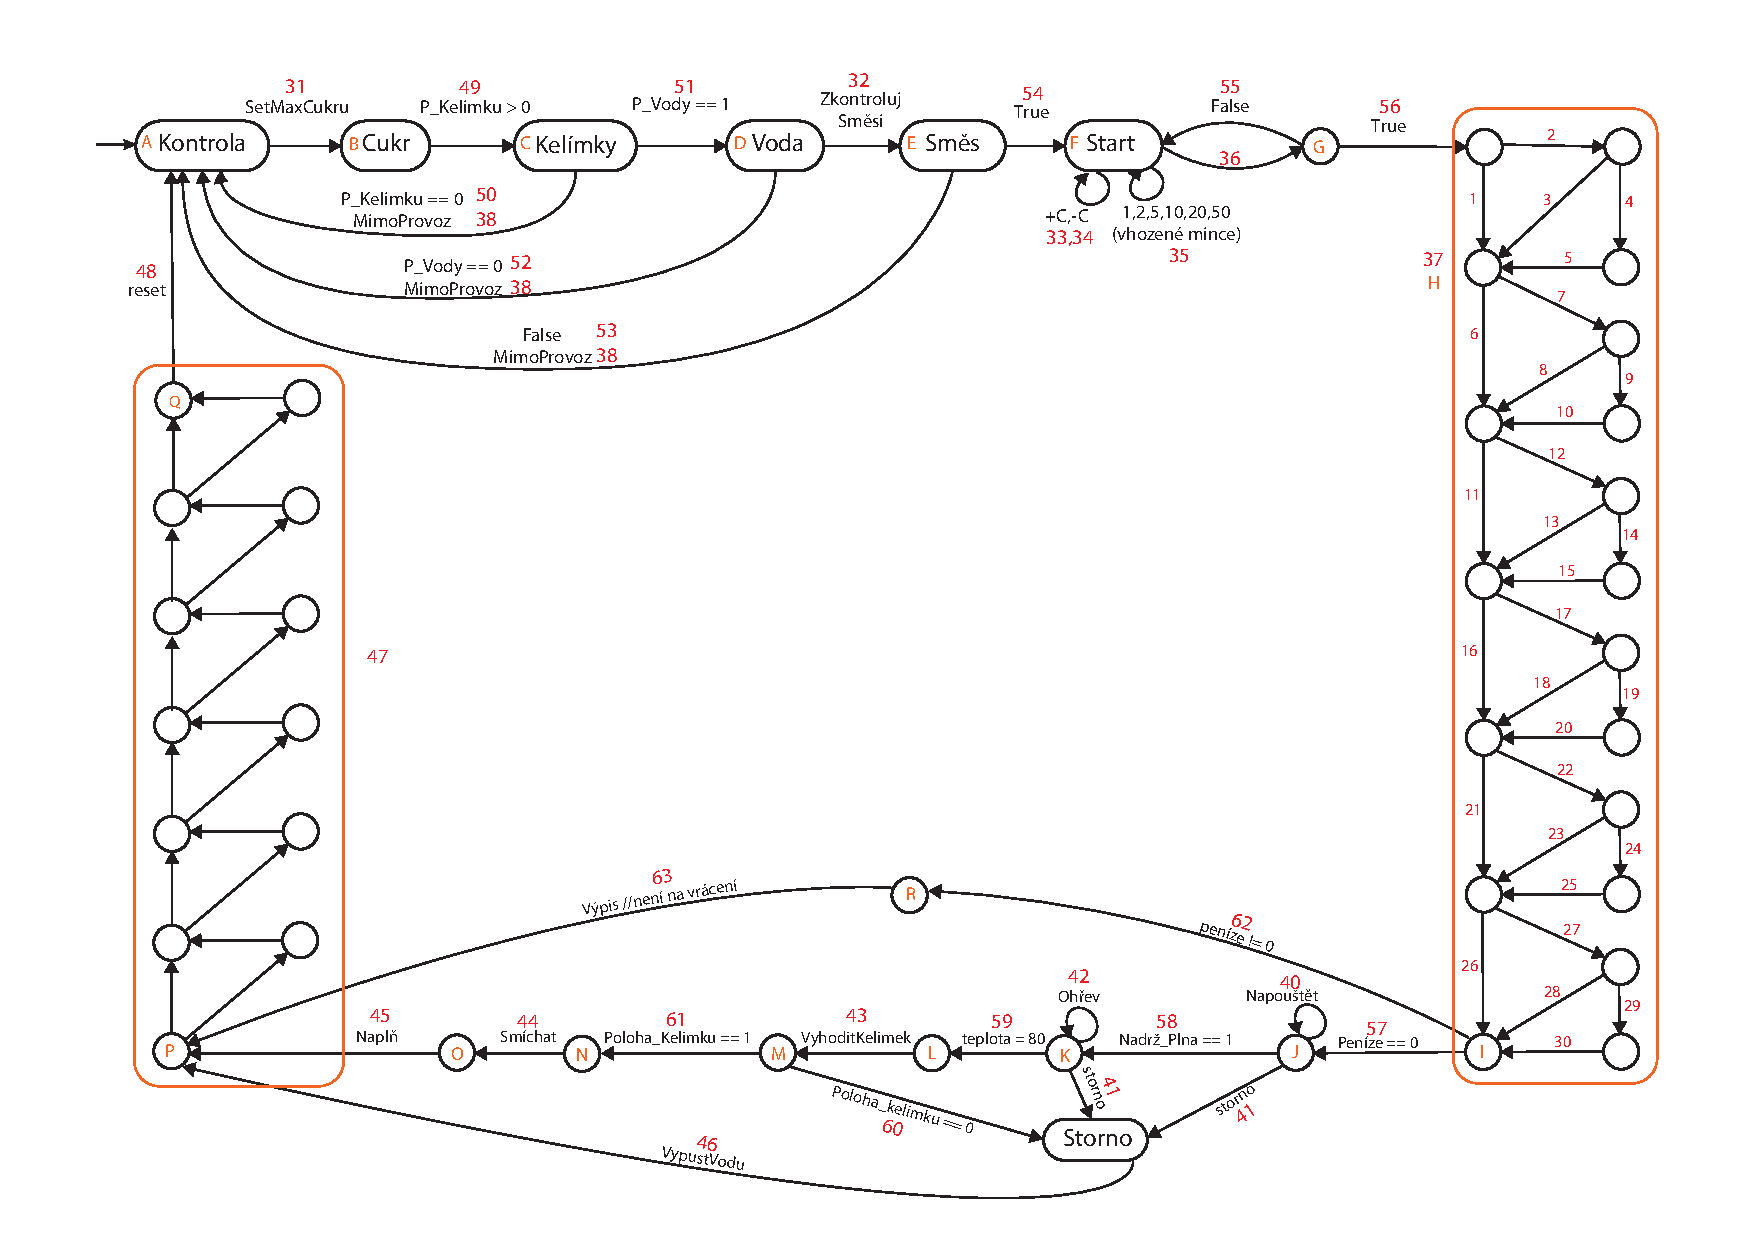
\includegraphics[angle=-90,width=\textwidth]{doc/kavovar_KA.pdf}
	\caption{Nákres konečného automatu}
\end{figure}
	
\paragraph{\parindent=4em}{	
	Stavy mezi H a I zajišťují převedení přeplatku na mince, které má automat k dispozici. Nejprve se testuje, jestli lze přeplatek vrátit v mincích hodnoty 50 Kč, pokud je to možné, automat spočte, kolik takových mincí může vrátit. Poté odečte částku, kterou vrátí v těchto mincích od celkového přeplatku a pokračuje mincemi hodnoty 20 Kč. Pokud automat nemůže částku vrátit v mincích hodnoty 50 Kč, přejde rovnou na mince hodnoty 20 Kč a takto pokračuje až po hodnotu 1 Kč. Pokud nastane situace, že automat dojde do stavu I a přeplatek nebude 0 Kč, automat nemá na vrácení a přejde do stavu, kdy vrátí uživateli vhozenou částku.
}	

\paragraph{\parindent=4em}{	
	Stavy mezi P a Q zajišťují vrácení přeplatku. O to, které mince musí automat zákazníkovi vrátit se starají stavy mezi stavem H a I. Mechanismus je podobný tomu, který zjišťuje jaké mince vrátit. Nejprve automat testuje, jestli má nějaké mince hodnoty 50 Kč k vrácení, pokud ano, vrátí zákazníkovi vypočtený počet mincí této hodnoty, poté přejde na mince hodnoty 20 Kč. Když automat nemá vracet žádné mince hodnoty 50 Kč, zkusí jestli má vrátit mince hodnoty 20 Kč atd..
}	

\begin{figure}[H]	
	\centering
	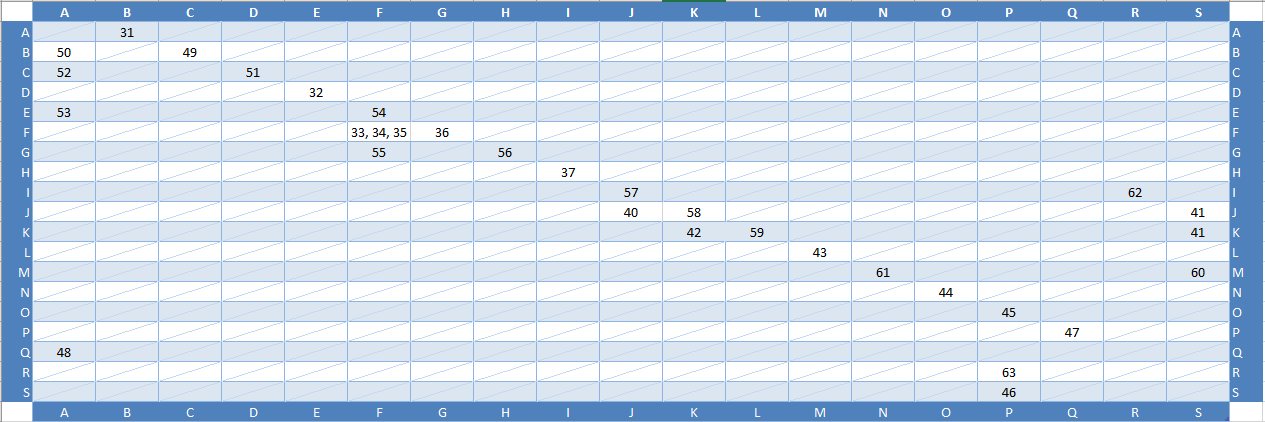
\includegraphics[width=\textwidth]{images/tabulka_prechodovych_funkci}
	\caption{Tabulka přechodových funkcí KA}
\end{figure}

\section{Implementace}

\paragraph{\parindent=4em}{	
	Nápojový automat je implementován v jazyce Java. Celá aplikace funguje v konzolovém režimu. V hlavním konstruktoru se nastaví všechny důležité parametry pro chod automatu např. přísun vody, počet kelímků, počet nápojových směsí atd. V aplikační třídě se tedy vytvoří instance tohoto automatu a nad touto instancí zavoláme metodu {\it startKA()} na spuštění automatu. V této metodě si nastavíme proměnnou {\it stav} na výchozí stav {\it A}. Dále metoda pokračuje do cyklu {\it while}, v kterém je {\it switch}, který přepíná mezi stavy. Ve stavu {\it F} očekáváme vstup od uživatele. Ze stavu {\it Q} se automat znovu přepne do výchozího stavu {\it A}.
}

\section{Testování automatu}

\subsection{Testovací data}

\paragraph{\parindent=4em}{	
	K testování automatu jsme použili automaticky generovaná data třídy {\it Gen\_dat}. Tato třída generuje data tak, že projde všechny stavy automatu, jelikož těchto dat je obrovské množství, omezili jsme každý vstup na maximálně 3 různé hodnoty. Další omezení dat jsme provedli snížením počtu iterací vhození mincí, když je automat ve stavu mimo provoz.
	
	Pro zautomatizování testování jsme museli pozměnit chod automatu, např.: automat skončí po jednom cyklu. Tyto změny jsou jen při testování.
}

\paragraph{\parindent=4em}{	
	Vygenerovaná testovací data jsou ve formátu {\it .txt} a mají tuto strukturu:\\
}

\begin{figure}[H]	
	\centering
	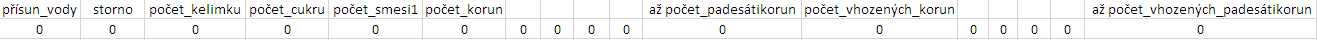
\includegraphics[width=\textwidth]{images/format}
	\caption{Formát generovaných dat}
\end{figure}

\paragraph{\parindent=4em}{	
	Výstupem testu je text, kde na každé řádce je příslušný výpis automatu k řádce testovacích dat, jednotlivé výstupy jsou odděleny čárkou.
}

\subsection{Spuštění automatického testování}

\paragraph{\parindent=4em}{	
	V adresáři {\it test/tester/bin} se nachází script pro spuštění automatických testů {\it test.cmd}.
}

\section{Struktura adresáře}

\begin{figure}[H]	
	\centering
	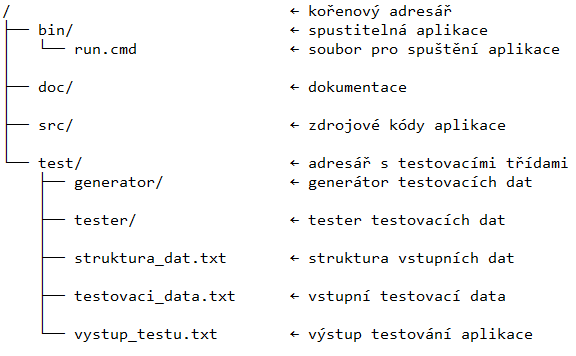
\includegraphics[width=\textwidth]{images/adresar}
	\caption{Adresářová struktura}
\end{figure}

\section{Uživatelská příručka}

\subsection{Spuštění aplikace}

\paragraph{\parindent=4em}{	
	Aplikace se spouští souborem {\it run.cmd} v adresáři {\it bin}.
}

\subsection{Po spuštění}

\paragraph{\parindent=4em}{	
	Po spuštění aplikace se uživateli zobrazí zda chce zadat interní vstupy, může se rozhodnout pomocí kláves {\it y/n}. Pokud stiskne {\it n}, automat se spustí s přednastavenými interními vstupy. V případě, že uživatel zadá {\it y}, musí nejprve zadat všechny interní vstupy, bez kterých se nemůže automat spustit. Poté se zobrazí stručný návod jak aplikaci používat viz obr. \ref{fig:pospusteni}. Automat vypisuje 2 druhy zpráv, interní a externí. Interní jsou v hranatých závorkách.
}

\begin{figure}[H]	
	\centering
	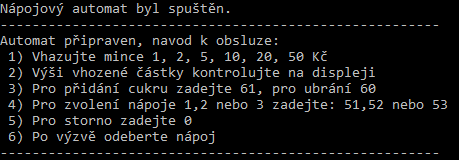
\includegraphics[width=\textwidth]{images/spusteni}
	\caption{Stručný návod po spuštění}
	\label{fig:pospusteni}
\end{figure}

\subsection{Ovládání}

\paragraph{\parindent=4em}{	
	Aplikace se ovládá pomocí klávesnice, zadáním příslušného vstupu pro operaci.
}

\newpage
\section{Závěr}

\paragraph{\parindent=4em}{	
	Podle zadání jsme vytvořili návrh konečného automatu pro nápojový automat, který jsme posléze implementovali jako konzolovou aplikaci. Při vytváření aplikace vznikly nesrovnalosti mezi návrhem konečného automatu a implementací z důvodu jednoduššího zapsání algoritmu pro vracení přeplatku. Dále jsme museli pozměnit chod automatu, kvůli zautomatizování testování aplikace.
}

%
%	KONEC
%
\end{document}
